Polynomilausekkeiden käsittely on välttämätön taito matematiikassa, ja siksi tähän lukuun kannattaa paneutua huolella.

Polynomeja voidaan reaalilukujen osittelulain nojalla kertoa vakiolla kertomalla kukin termi erikseen.

\begin{esimerkki}
	Olkoon $P(x)=x^3-2x^2+1$. Määritä lausekkeen $4P(3)$ arvo.
	\begin{esimratk}
	(TAPA 1.)
		Polynomi $P(x)$ kerrotaan vakiolla $4$ kertomalla kukin termi erikseen.
		\begin{align*}
		 4P(x)&=4(x^3-2x^2+1)\\
		 &=4x^3-4\cdot2x^2+4\cdot1\\
		 &=4x^3-8x^2+4.
		\end{align*}
		
		Määritetään polynomin $4P(x)$ arvo, kun $x=3$
		\begin{align*}
		 4P(3)&=4\cdot3^3-8\cdot3^2+4\\
			&=4\cdot27-8\cdot9+4\\
			&=108-72+4\\
			&=40.
		\end{align*}
	(TAPA 2.)
		Ratkaistaan ensin $P(3)$, ja kerrotaan se vasta sen jälkeen vakiolla $4$.
		\begin{align*}
		 P(3)&=3^3-2\cdot3^2+1\\
			&=27-2\cdot9+1\\
			&=27-18+1\\
			&=10,
		\end{align*}
		jolloin $4P(3)=4\cdot10=40$.
	\end{esimratk}
	\begin{esimvast}
	 $4P(3)=40$.
	\end{esimvast}
\end{esimerkki}

\subsection{Polynomien yhteen- ja vähennyslasku}

\qrlinkki{http://opetus.tv/maa/maa2/polynomien-yhteen-ja-vahennyslasku/}
{Opetus.tv: \emph{polynomien yhteen- ja vähennyslasku} (7:36)}

Kaikkien polynomien summat ja erotukset ovat aina polynomeja. Polynomeja voidaan laskea yhteen yhdistämällä samanasteiset termit. On kätevää aloittaa ryhmittelemällä samanasteiset termit vierekkäin. Polynomit sievennetään yleensä aina yleiseen muotoon asti, jossa on vain yksi termi kutakin astetta kohti.

Samanasteisten termien yhteen- ja vähennyslasku perustuu siihen, että soveltamalla reaalilukujen osittelulakia $a(b\pm c)=ab\pm ac$ oikealta vasemmalle (ks. Vapaa matikka 1) samanasteiset potenssit voidaan ottaa yhteiseksi tekijäksi:

\[ ax^n \pm bx^n = (a \pm b)x^n \]

\begin{esimerkki}

	\begin{itemize}
	\item $2x+3x=(2+3)x=5x$
	\item $t-5t=1t-5t=(1-5)t=-4t$
	\item $5,1k^2+3,04k^2 = (5,1+3,04)k^2 = 8,14k^2$
	\item $\frac{1}{2}y^{42}+\frac{1}{3}y^{42}=(\frac{1}{2}+\frac{1}{3})y^{42}= (\frac{3}{6}+\frac{2}{6})y^{42}=\frac{3+2}{6}y^{42}=\frac{5}{6}y^{42}$
	\end{itemize}
\end{esimerkki}

\begin{esimerkki}
Laske polynomien $5x^2-x+5$ ja $3x^2-1$ summa.
    \begin{esimratk}
    
        \begin{align*}
            (\textcolor{blue}{5x^2} \textcolor{red}{{}-x} + 5) + (\textcolor{blue}{3x^2} -1) 
            &=\textcolor{blue}{5x^2} \textcolor{red}{{}-x} + 5 + \textcolor{blue}{3x^2} -1 \\
            &=\textcolor{blue}{5x^2+3x^2} \textcolor{red}{{}-x} +5-1\\
%                       &=\textcolor{blue}{(5+3)x^2} \textcolor{red}{{}-x}+(5-1)\\
            &=\textcolor{blue}{8x^2} \textcolor{red}{{}-x}+4.
        \end{align*}     
    \end{esimratk}
    \begin{esimvast}
        Polynomien summa on $8x^2-x+4$.
    \end{esimvast}
\end{esimerkki}

Edellisessä esimerkissä molemmat yhteenlaskettavat polynomit laitettiin rakenteen selventämisen vuoksi kaarisulkeiden sisään, vaikka niillä ei ollutkaan laskujärjestyksen kannalta mitään merkitystä.

Polynomeja voidaan vastaavalla tavalla vähentää toisistaan. Vähennyslaskun tapauksessa on tärkeää laittaa vähennettävä polynomi sulkeisiin, sillä miinusmerkki vaikuttaa \emph{koko} polynomiin, ei vain sen ensimmäiseen termiin. Sulkeet avattaessa pitää muistaa vaihtaa kaikkien termien merkki: 

\begin{esimerkki}
    Laske polynomien $4x^3+1$ ja $6x^3-2$ erotus.
    \begin{esimratk}
        \begin{align*}
		(\textcolor{blue}{4x^3}+1)-(\textcolor{blue}{6x^3}-2) \\
		&= \textcolor{blue}{4x^3}+1 - \textcolor{blue}{6x^3} -(-2) \\
		&= \textcolor{blue}{4x^3}+1 - \textcolor{blue}{6x^3} + 2 \\
		&= \textcolor{blue}{4x^3-6x^3} +1 +2 \\
		&=\textcolor{blue}{-2x^3}+3
        \end{align*}
    \end{esimratk}
    \begin{esimvast}
        Polynomien erotus on $-2x^3+3$.
    \end{esimvast}
\end{esimerkki}

\begin{esimerkki}
    Laske polynomien $14x^3+69$ ja $3x^3+2x^2+x$ erotus.
    \begin{esimratk}
        \begin{align*}
            (\textcolor{blue!30!green}{14x^3} + 69) - (\textcolor{blue!30!green}{3x^3} \textcolor{blue}{{}+ 2x^2} \textcolor{red}{{}+x})
            &= \textcolor{blue!30!green}{14x^3} + 69 \textcolor{blue!30!green}{{}-3x^3} \textcolor{blue}{-2x^2} \textcolor{red}{{}-x} \\
            &= \textcolor{blue!30!green}{14x^3{}-3x^3} \textcolor{blue}{{}-2x^2} \textcolor{red}{{}-x} + 69 \\
%           &= \textcolor{blue!30!green}{(14{}-3)x^3} \textcolor{blue}{{}-2x^2} \textcolor{red}{{}-x} + 69 \\
            &= \textcolor{blue!30!green}{11x^3} \textcolor{blue}{{}-2x^2} \textcolor{red}{{}-x} + 69
        \end{align*}
    \end{esimratk}
    \begin{esimvast}
        Polynomien erotus on $11x^3-2x^2-x+69$.
    \end{esimvast}
\end{esimerkki}

\begin{esimerkki}
    Olkoot polynomit $P(x)=2x+1$ ja $Q(x)=3x^2-2x+5$. Määritä summa $R(x)=P(x)+Q(x)$.
    \begin{esimratk}
        \begin{align*}
            R(x) = P(x)+Q(x) &= (2x+1)+(3x^2-2x+5) \\
                             &= 2x+1+3x^2-2x+5 \\
                             &= 3x^2+2x-2x+1+5 \\
                             &= 3x^2+6.
        \end{align*}
    \end{esimratk}
    \begin{esimvast}
        $R(x) = 3x^2+6$.
    \end{esimvast}
\end{esimerkki}

\begin{esimerkki}
    Laske polynomien $P$ ja $Q$ erotus $R$, kun $P(x)=-3x^4+x^2+1$ ja $Q(x)=-3x^4+3x^3-x$.
    Mikä on polynomin $R$ aste?
   \begin{esimratk}
        \begin{align*}
            R(x) = P(x)-Q(x) &= (-3x^4+x^2+1)-(-3x^4+3x^3-x) \\
                             &= -3x^4+x^2+1+3x^4-3x^3+x \\
                             &= -3x^4+3x^4-3x^3+x^2+x+1 \\
                             &= -3x^3+x^2+x+1.
        \end{align*}
    \end{esimratk}
    \begin{esimvast}
        $R(x) = -3x^3+x^2+x+1$. Polynomin $R$ aste on kolme.
    \end{esimvast}
\end{esimerkki}

\subsection{Polynomien kertolasku}

\qrlinkki{http://opetus.tv/maa/maa2/polynomien-kertolasku/}
{Opetus.tv: \emph{polynomien kertolasku} (10:00)}

\subsubsection*{Monomien tulo}

Kahden monomin tulo sievennetään kertomalla kertoimet keskenään ja kirjainosat keskenään. Muista potenssien laskusäännöt (ks. Vapaa matikka 1)!

\begin{esimerkki}
    Laske \quad 
    a) $2x\cdot 3x$ \quad
    b)$-3x^2\cdot (-5x^4)$ \quad
    c) $5x^2 \cdot (-2x)$
    \begin{esimratk}
        \begin{alakohdat}
            \alakohta{$2x\cdot 3x = 2\cdot 3\cdot x\cdot x = 6x^2$}
            \alakohta{$-3x^2\cdot (-5x^4) = (-3)\cdot (-5) \cdot x^2 \cdot x^4 = 15 x^6$}
            \alakohta{$5x^2 \cdot (-2x) = -10 x^3$}
        \end{alakohdat}
    \end{esimratk}
    \begin{esimvast}
        a) $6x^2$ \quad
        b) $15x^6$ \quad
        c) $-10x^3$
    \end{esimvast}
\end{esimerkki}

\subsubsection*{Polynomin kertominen monomilla}

Polynomeja voi kertoa keskenään reaalilukujen tuttujen laskusääntöjen avulla. Yksinkertaisin erikoistapaus on polynomin kertominen monomilla, jolloin
käytetään osittelulakia $a(b+c)=ab+ac$.

\begin{esimerkki}
Laske \quad a) $5\cdot(x+3)$ \quad b) $2x(x-5)$ \quad 
c) $3(a+b+c)$
\begin{alakohdat}
    \alakohta{$5\cdot(x+3) = 5\cdot x + 5\cdot 3 = 5x+15$}
    \alakohta{$2x(x-5)=2x\cdot x -2\cdot x \cdot 5 = 2x^2-10x$}
    \alakohta{$3(a+b+c)=3a+3b+3c$}
\end{alakohdat}
\end{esimerkki} 

\subsubsection*{Kahden binomin tulo}

Kahden binomin tulon laskusääntö perustellaan soveltamalla osittelulakia kahdesti:

\begin{align*}
(a+b)(c+d) &= (a+b)\cdot c + (a+b)\cdot d &\emph{osittelulaki} \\
 &= ac+bc+ad+bd &\emph{osittelulaki} 
\end{align*}

Kahden binomin tulossa siis kummallakin ensimmäisen binomin termillä kerrotaan toisen binomin termit. Saadut neljä tuloa lasketaan yhteen. 

\newcommand{\pbezier}[4]{
	\pgfmathsetmacro{\PBxa}{#1}
	\pgfmathsetmacro{\PBxb}{#2}
	\pgfmathsetmacro{\PBya}{#3}
	\pgfmathsetmacro{\PByb}{#3+#4}
	\pgfmathsetmacro{\PBca}{0.8 * \PBxa + 0.2 * \PBxb}
	\pgfmathsetmacro{\PBcb}{0.2 * \PBxa + 0.8 * \PBxb}
	\draw[color=red] (\PBxa, \PBya) .. controls (\PBca, \PByb) and (\PBcb, \PByb) .. (\PBxb, \PBya);
}

\begin{esimerkki}
Laske binomien $x+2$ ja $x-5$ tulo. \\
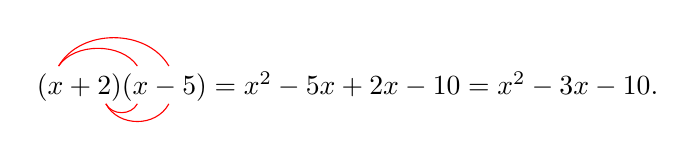
\begin{tikzpicture}
\draw node[right] {$(x+2)(x-5) = x^2-5x+2x-10 = x^2 -3x-10.$};

\pgfmathsetmacro{\klAx}{0.40}
\pgfmathsetmacro{\klBx}{1.00}
\pgfmathsetmacro{\klCx}{1.4}
\pgfmathsetmacro{\klDx}{1.8} 
\pgfmathsetmacro{\klEx}{2.5}
\pgfmathsetmacro{\klLo}{-0.22}
\pgfmathsetmacro{\klHi}{0.26}

\pbezier{\klAx}{\klCx}{\klHi}{0.3}
\pbezier{\klAx}{\klDx}{\klHi}{0.48}

\pbezier{\klBx}{\klCx}{\klLo}{-0.15}
\pbezier{\klBx}{\klDx}{\klLo}{-0.3}
\end{tikzpicture}\newline
\end{esimerkki}

\begin{esimerkki}
Laske binomien $x^2-x$ ja $2x-1$ tulo. \\
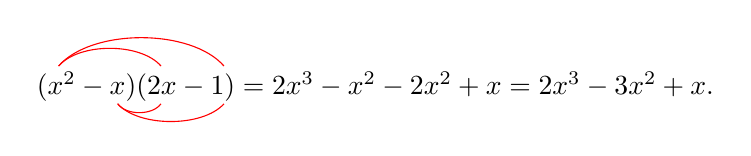
\begin{tikzpicture}
\draw node[right] {$(x^2-x)(2x-1) = 2x^3-x^2-2x^2+x = 2x^3 -3x^2 +x.$};

\pgfmathsetmacro{\klAx}{0.40}
\pgfmathsetmacro{\klBx}{1.15}
\pgfmathsetmacro{\klCx}{1.7}
\pgfmathsetmacro{\klDx}{2.5}
\pgfmathsetmacro{\klEx}{2.7}
\pgfmathsetmacro{\klLo}{-0.22}
\pgfmathsetmacro{\klHi}{0.26}

\pbezier{\klAx}{\klCx}{\klHi}{0.3}
\pbezier{\klAx}{\klDx}{\klHi}{0.48}

\pbezier{\klBx}{\klCx}{\klLo}{-0.15}
\pbezier{\klBx}{\klDx}{\klLo}{-0.3}
\end{tikzpicture}\newline
\end{esimerkki}




\subsubsection*{Yleinen kertolasku}

Osittelulain nojalla kahden polynomin tulo saadaan laskemalla yhteen kaikki
termit, jotka saadaan kertomalla termi ensimmäisestä ja toinen termi toisesta
polynomista.


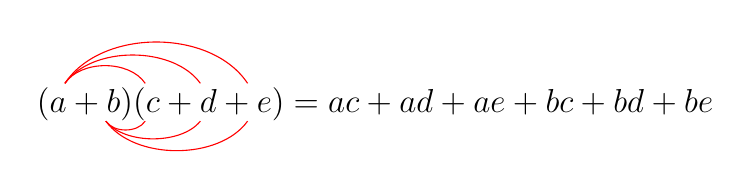
\begin{tikzpicture}
\draw node[right] {\large $(a+b)(c+d+e) = ac+ad+ae+bc+bd+be$};

\pgfmathsetmacro{\klAx}{0.48}
\pgfmathsetmacro{\klBx}{1.0}
\pgfmathsetmacro{\klCx}{1.5}
\pgfmathsetmacro{\klDx}{2.2}
\pgfmathsetmacro{\klEx}{2.8} %oli 3.26
\pgfmathsetmacro{\klLo}{-0.22}
\pgfmathsetmacro{\klHi}{0.26}

\pbezier{\klAx}{\klCx}{\klHi}{0.3}
\pbezier{\klAx}{\klDx}{\klHi}{0.48}
\pbezier{\klAx}{\klEx}{\klHi}{0.7}

\pbezier{\klBx}{\klCx}{\klLo}{-0.15}
\pbezier{\klBx}{\klDx}{\klLo}{-0.3}
\pbezier{\klBx}{\klEx}{\klLo}{-0.5}
\end{tikzpicture}

\begin{esimerkki}
Laske polynomien $x-3$ ja $x^2-4x+3$ tulo. \\
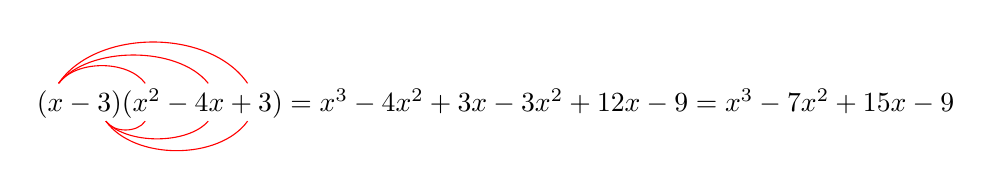
\begin{tikzpicture}
\draw node[right] {$(x-3)(x^2-4x+3) = x^3-4x^2+3x-3x^2+12x-9 = x^3-7x^2+15x-9$};

\pgfmathsetmacro{\klAx}{0.40}
\pgfmathsetmacro{\klBx}{1.00}
\pgfmathsetmacro{\klCx}{1.5}
\pgfmathsetmacro{\klDx}{2.3}
\pgfmathsetmacro{\klEx}{2.8}
\pgfmathsetmacro{\klLo}{-0.22}
\pgfmathsetmacro{\klHi}{0.26}

\pbezier{\klAx}{\klCx}{\klHi}{0.3}
\pbezier{\klAx}{\klDx}{\klHi}{0.48}
\pbezier{\klAx}{\klEx}{\klHi}{0.7}

\pbezier{\klBx}{\klCx}{\klLo}{-0.15}
\pbezier{\klBx}{\klDx}{\klLo}{-0.3}
\pbezier{\klBx}{\klEx}{\klLo}{-0.5}
\end{tikzpicture}\newline
\end{esimerkki}

\begin{esimerkki}
Laske polynomien $x^4-3x^3+3$ ja $x^3-2x^2+1$ tulo. \\
\begin{align*}
&\hspace{0.5cm}(\textcolor{red}{x^4} \textcolor{blue}{-3x^3} +{}\textcolor{blue!30!green}{3})(x^3-2x^2+1) \\
&= \textcolor{red}{x^4}\cdot x^3 + \textcolor{red}{x^4}\cdot (-2x^2)+\textcolor{red}{x^4}\cdot 1\textcolor{blue}{{}-3x^3}\cdot x^3\textcolor{blue}{{}-3x^3}\cdot(-2x^2)\textcolor{blue}{{}-3x^3}\cdot1 \\
&\hspace{0.5cm}+\textcolor{blue!30!green}{3}x^3+\textcolor{blue!30!green}{3}\cdot(-2x^2)+\textcolor{blue!30!green}{3}\cdot 1 \\
&= x^7-2x^6+x^4-3x^6+6x^5-3x^3+3x^3-6x^2+3 \\
&= x^7-5x^6+6x^5+x^4-6x^2+3
\end{align*}
\end{esimerkki}